
\documentclass[9pt,xcolor={svgnames}]{beamer}

\mode<presentation> {
\usetheme{default}
\usepackage{makecell}
\usepackage{threeparttable}  
\usepackage{tikz}
\usepackage{colortbl} % For coloring cells
\usepackage{pgfplots}
\pgfplotsset{compat = newest}
\usetikzlibrary{positioning, arrows.meta}
\usepgfplotslibrary{fillbetween}

\usetikzlibrary{positioning, arrows.meta}
\usepackage{natbib}
\bibliographystyle{plainnat}

%\setbeamertemplate{footline} % To remove the footer line in all slides uncomment this line
\setbeamertemplate{footline}[frame number] % To replace the footer line in all slides with a simple slide count uncomment this line
\setbeamertemplate{footline}
{
  \hfill%
  \usebeamercolor[fg]{page number in head/foot}%
  \usebeamerfont{page number in head/foot}%
%  \insertframenumber\,/\,\inserttotalframenumber\kern1em\vskip2pt % original code
  \tiny % font size: tiny(default)/scriptsize/footnotesize/small/normalsize/large
  \insertframenumber
  \kern1em  % adjust the space on the right-hand side of the frame number
  \vskip4pt % adjust the space below the frame number
}

\setbeamertemplate{navigation symbols}{} % To remove the navigation symbols from the bottom of all slides uncomment this line
}

\usepackage{graphicx} % Allows including images
\usepackage{booktabs} % Allows the use of \toprule, \midrule and \bottomrule in tables
\usepackage{multicol}
\usepackage{mathtools}
\usepackage{geometry}
\usepackage{bbm}

\usepackage[export]{adjustbox}


\setbeamertemplate{caption}[numbered]
\setbeamertemplate{itemize items}[circle]
\setbeamertemplate{itemize subitem}[default]
%\setbeamertemplate{enumerate items}[circle]\\
%\setbeamertemplate{items}[circle]

%\setbeamercolor{item}{fg=black} % all frames will have bullets with this color
%\setbeamercolor{caption name}{fg=gray} % all frames will have captions with this color

\usefonttheme[onlymath]{serif}

\setlength{\leftmargini}{9pt}
\setbeamersize{text margin left=20pt,text margin right=20pt}
%\setbeamerfont{institute}{size=\normalsize}

\setbeamertemplate{frametitle}
{
{\vskip  .6em} 
{\hskip -.35em}
\underline{\insertframetitle\vphantom{j}}
{\vskip -.6em}
}

\graphicspath{{./figs181007/}}


%----------------------------------------------------------------------------------------
%   TITLE PAGE
%----------------------------------------------------------------------------------------

\title[Bridging the Manufacturing Gap]{\large \textbf{Sectoral Employment Share under Labor Search Frictions\\ \normalsize A search-and-matching view of industrialization and the manufacturing gap}}
\author{Shisham Adhikari\thanks{University of California – Davis; \texttt{shadhikari@ucdavis.edu}} \and Si Guo\thanks{International Monetary Fund; \texttt{sguo@imf.org}}}

\date[Davis]{%
  UC Davis Development Tea\\[0.5em]
  \today
}

\begin{document}

\begin{frame}
\titlepage % Print the title page as the first slide
\end{frame}

    %===============================================


\section{Past} 
\begin{frame}{Motivation: A Circular challenge in industrialization}

% tighten the space between columns
\setlength{\columnsep}{8pt}

\begin{columns}[T,onlytextwidth]
% ---- Left: text ----
\begin{column}{0.62\textwidth}
 \begin{itemize}
    \item \textbf{Circular challenge in manufacturing expansion:} 
    \begin{itemize}
        \item Firms report a shortage of right skilled workers.
        \item Workers report a lack of manufacturing jobs.
    \end{itemize}
    
    \vspace{4mm}

    \item This circular pattern raises questions about market failures and policy intervention. 
    
    \vspace{4mm}
    
    \item \textbf{Many countries started initiatives to develop (often high-tech) manufacturing sectors,} 
    many of them also cover STEM education and training.
    \begin{itemize}
        \item China: Made in China 2025
        \item US: CHIPS Act; Manufacturing USA
        \item Korea: Manufacturing 4.0 
        \item Germany: Industrie 4.0
    \end{itemize}
  \end{itemize}
\end{column}

% ---- Right: tight cycle chart ----
\begin{column}{0.38\textwidth}
\vspace*{6mm} % push the figure down a bit
\begin{tikzpicture}[
  >=Latex,
  every node/.style={font=\scriptsize, text=structure.fg},
  line width=0.9pt,
  baseline
]
  % radii: arrows (R) and labels (T)
  \def\R{1.05}
  \def\T{1.60}

  % arrows (clockwise)
  \draw[->, draw=structure.fg] (180:\R) arc[start angle=180, end angle=90,  radius=\R];
  \draw[->, draw=structure.fg] ( 90:\R) arc[start angle=90,  end angle=0,   radius=\R];
  \draw[->, draw=structure.fg] (  0:\R) arc[start angle=0,   end angle=-90, radius=\R];
  \draw[->, draw=structure.fg] (-90:\R) arc[start angle=-90, end angle=-180,radius=\R];

  % labels
  \node[yshift=-1.2mm] at (90:\T)  {Less value to firms};
  \node[xshift=1mm]     at (  0:\T)  {Fewer firms};
  \node[yshift=1.2mm]   at (-90:\T)  {Less value to workers};
  \node[xshift=-2mm]    at (180:\T) {Fewer workers};
\end{tikzpicture}

\begin{flushright}
  {\tiny\emph{Chicken-and-egg cycle in manufacturing expansion}}
\end{flushright}
\end{column}
\end{columns}

\vspace{4mm}
\small
\textit{This paper formalizes this circular pattern in a two-sector search-and-matching labor model.}

\end{frame}


\begin{frame}{Motivation: Firms report shortage of workers}
  \begin{figure}
    \centering
    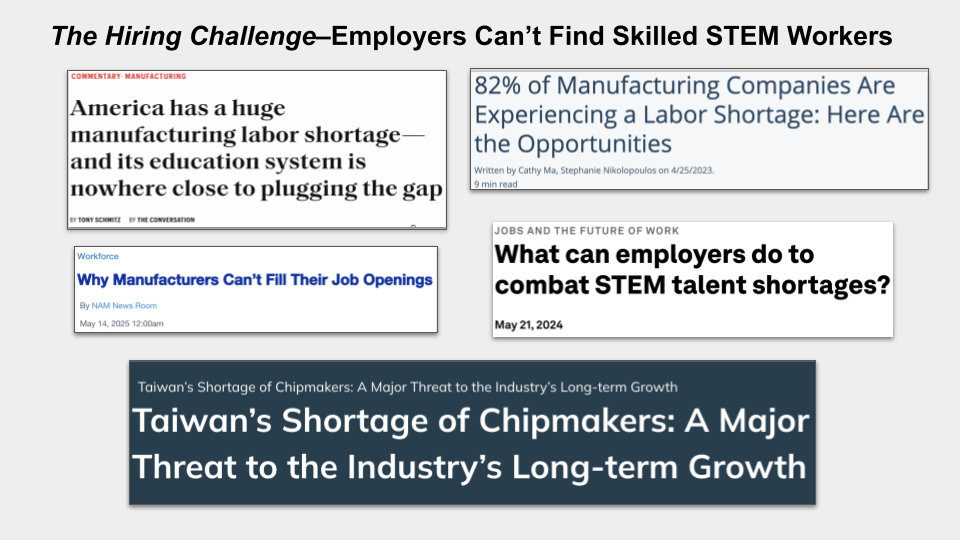
\includegraphics[width=1\textwidth]{figures/employers.png}
    \label{fig:empirics}
  \end{figure}


\end{frame}

\begin{frame}{Motivation: Workers report shortage of jobs}
  \begin{figure}
    \centering
    
\includegraphics[width=1\textwidth]{figures/employees.png}
    \label{fig:empirics}
  \end{figure}
\end{frame}

% ===================== WHAT DO WE DO =====================
\begin{frame}{What do we do?}
\begin{itemize}
  \item \textbf{Question}
  \begin{itemize}
      \item Should governments actively support manufacturing and/or STEM education?
      \item If yes, \textbf{where} should policy act? On firms’ investment? On workers’ training?
  \end{itemize}
  \vspace{2em}
  \item \textbf{Answers}
    \begin{itemize}
      \item Labor market frictions + higher capital intensity in manufacturing 
      \item If the \textit{Hosios condition} holds\footnote{Hosios condition is a standard efficiency condition that corrects search externalities in search-and-matching models.}:
      \begin{itemize}
          \item Search externalities are corrected; only capital inefficiency remains
          \item $\Rightarrow$ \textbf{Subsidize firms} (capital / vacancies in manufacturing)
      \end{itemize}
      \item If the Hosios condition does \textit{not} hold:
        \begin{itemize}
          \item There is an additional distortion against manufacturing on the worker side
          \item $\Rightarrow$ \textbf{Subsidize both workers and firms}
      \end{itemize}
    \end{itemize}
\end{itemize}
\end{frame}


% ===================== HOW DO WE DO IT =====================

\begin{frame}{Outline}
\begin{itemize}
    \item \textbf{Empirics:}  
    Cross-country patterns in STEM enrollment and industry employment

    \medskip

    \item \textbf{Theory:}  
    A two-sector model (manufacturing $m$ and services $s$) 
    with search frictions and endogenous capital

    \medskip

    \begin{itemize}
        \item Inefficiency: decentralized equilibrium (DE) vs. social planner (SP)
        \vspace{2mm}
        \item Policy mapping 
    \end{itemize}

    \medskip

    \item \textbf{Quantitative Results:}  
    calibration to an “average” emerging market (EM)

       \begin{itemize}
        \item 
        \item 
    \end{itemize}

    
\end{itemize}
\end{frame}


\begin{frame}
\frametitle{Data Source for the Stylized Empirical Motivation}
\begin{itemize}

\item \textbf{UNESCO (UIS):} Tertiary enrollment by field, 1999–2023. 
STEM = \textbf{ICT, Natural Sciences, and Engineering}.  
For each country, we take the \textbf{earliest available year} to approximate \textbf{initial STEM supply}.

\medskip

\item \textbf{Groningen Growth and Development Centre (GGDC, 10-sector / Structural Change):} 
Employment and value added, latest available year (2018 for most; 2011 for some).  
“\textbf{Industry}” $=$ mining $+$ utilities $+$ manufacturing $+$ construction.

\end{itemize}
\end{frame}



\begin{frame}{Tertiary Enrollment by Field (\% of total) in 2019}
\begin{center}
%\textbf{\large Higher Education Enrollment Distribution by Fields}

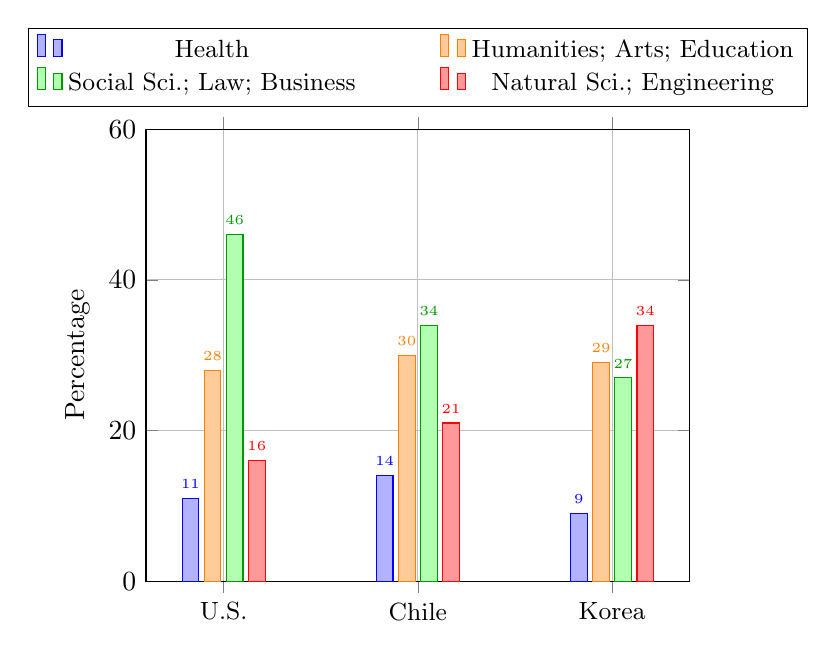
\begin{tikzpicture}
\begin{axis}[
    width=0.7\linewidth,
    ybar,
    bar width=6pt,
    ylabel={Percentage},
    symbolic x coords={U.S., Chile, Korea},
    xtick=data,
    ymin=0,
    ymax=60,
    enlarge x limits=0.2,
    legend style={
        at={(0.5,1.05)},
        anchor=south,
        legend columns=2,
        font=\small,
        /tikz/every even column/.append style={column sep=1cm}
    },
    grid=major,
    nodes near coords,
    every node near coord/.append style={font=\tiny},
    ymajorgrids=true,
    xticklabel style={font=\small},
]

% Health (blue)
\addplot+[style={blue,fill=blue!30}] coordinates {
    (U.S.,11) (Chile,14) (Korea,9)
};

% Humanities, Arts, Education (orange)
\addplot+[style={orange,fill=orange!40}] coordinates {
    (U.S.,28) (Chile,30) (Korea,29)
};

% Social Sci., Law, Business (green)
\addplot+[style={green!60!black,fill=green!30}] coordinates {
    (U.S.,46) (Chile,34) (Korea,27)
};

% Natural Science, Engineering (red)
\addplot+[style={red,fill=red!40}] coordinates {
    (U.S.,16) (Chile,21) (Korea,34)
};

\legend{
    Health, Humanities; Arts; Education,
    Social Sci.; Law; Business, Natural Sci.; Engineering
}
\end{axis}
\end{tikzpicture}
\end{center}

\begin{center}
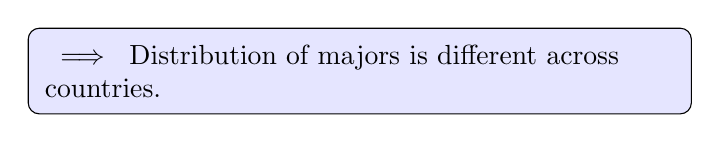
\begin{tikzpicture}
    \node[
        draw,
        rectangle,
        rounded corners,
        fill=blue!10,
        text width=8cm,
        align=left,   % <-- left-align text and let it fill the width
        inner sep=6pt
    ] (box) {
        $\implies$ Distribution of majors is different across countries.
    };
\end{tikzpicture}
\end{center}
\end{frame}

\begin{frame}{Countries with Higher STEM Shares Tend to Have Higher Industry Emp.}
\begin{figure}[htbp]
    \centering
    \caption{STEM share vs. industrial employment share.}
    \label{fig:stem_ind}
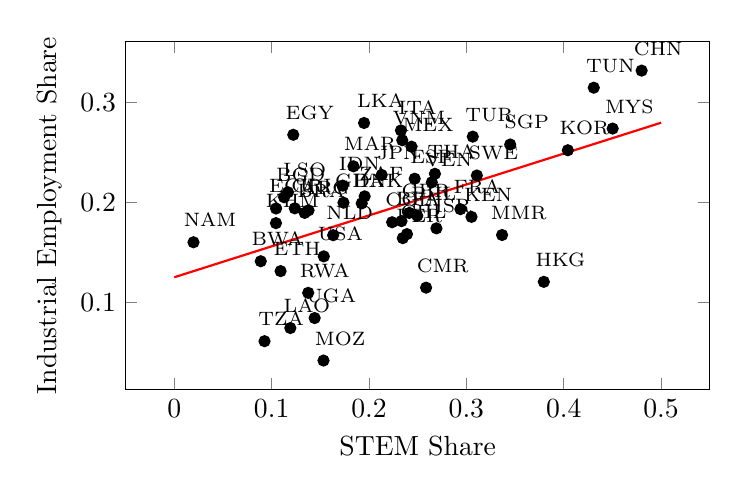
\begin{tikzpicture}
  \begin{axis}[
    width=9cm,
    height=6cm,
    % title={Relationship between STEM Share and Industrial Employment},
    xlabel={STEM Share},
    ylabel={Industrial Employment Share},
    ytick distance=0.1,  
    enlargelimits=0.1,
    scatter/classes={
        a={mark=o,draw=blue}
    },
    every node near coord/.append style={font=\scriptsize} % smaller font for country labels
  ]

    % Scatter points with country names as labels
  \addplot[
  scatter,
  only marks,
  scatter src=explicit symbolic,
  nodes near coords,
  nodes near coords align={center},
  nodes near coords style={font=\scriptsize, yshift=8pt, xshift=6pt} % shift label above marker
]
    coordinates {
 (0.1378744,0.1921153)[ARG]
  (0.2333404,0.1812904)[BFA]
  (0.1127611,0.2052854)[BGD]
  (0.1339324,0.1895628)[BRA]
  (0.0887872,0.1410377)[BWA]
  (0.2389722,0.1682635)[CHL]
  (0.48,0.3322481)[CHN]
  (0.2586084,0.1145408)[CMR]
  (0.223719,0.1801721)[COL]
  (0.1237097,0.194118)[CRI]
  (0.1925061,0.1990896)[DNK]
  (0.1045007,0.193951)[ECU]
  (0.122197,0.2678931)[EGY]
  (0.2469077,0.223834)[ESP]
  (0.1091694,0.1311437)[ETH]
  (0.2938787,0.1932734)[FRA]
  (0.2413404,0.1895179)[GBR]
  (0.1737703,0.1997761)[GHA]
  (0.3795342,0.1203752)[HKG]
  (0.1730061,0.2169031)[IDN]
  (0.2692143,0.1740516)[ISR]
  (0.2328073,0.2722787)[ITA]
  (0.213,0.2275904)[JPN]
  (0.3052545,0.1855444)[KEN]
  (0.104402,0.1792649)[KHM]
  (0.4042146,0.2523832)[KOR]
  (0.1191805,0.0740409)[LAO]
  (0.1948983,0.2797219)[LKA]
  (0.116723,0.2102498)[LSO]
  (0.1840243,0.2362694)[MAR]
  (0.2436201,0.2559769)[MEX]
  (0.336678,0.1673723)[MMR]
  (0.1532314,0.0414321)[MOZ]
  (0.4502603,0.2741223)[MYS]
  (0.0197044,0.1600689)[NAM]
  (0.1631535,0.1671708)[NLD]
  (0.2346783,0.1642373)[PER]
  (0.2495234,0.1866893)[PHL]
  (0.1375139,0.1093415)[RWA]
  (0.3450148,0.2581424)[SGP]
  (0.3107809,0.2270485)[SWE]
  (0.2676974,0.228728)[THA]
  (0.4308376,0.3151194)[TUN]
  (0.3065551,0.2660213)[TUR]
  (0.0926554,0.0608464)[TZA]
  (0.1441461,0.0840602)[UGA]
  (0.1535388,0.1459264)[USA]
  (0.2644799,0.2202186)[VEN]
  (0.2341544,0.2624081)[VNM]
  (0.1955149,0.206129)[ZAF]
    };

    % Trend line (replace slope/intercept with your regression results)
    \addplot[red, thick, mark=none, domain=0:0.5] {0.31*x + 0.125};
   % \addlegendentry{Trend line (yhat)}

  \end{axis}
\end{tikzpicture}

    \begin{minipage}{0.7\textwidth}  % Adjust width to match figure
        \footnotesize
        \textbf{Note:} STEM share is calculated as the annual number of tertiary graduates in STEM fields divided by total number of tertiary graduates. Industrial employment share is calculated as the number of employees in the industry sector divided by total employment.
    \end{minipage}
    
\end{figure}
\end{frame}


\begin{frame}{Industry Employment Share Correlates STEM enrollment Share}
\vspace{-1em}
\begin{align*}\label{regression}
    S_i = \beta_{stem} STEM_i + \delta \cdot X_i + \epsilon_i
\end{align*}

\vspace{-1em}

\begin{table}[htbp]
\centering
\begin{threeparttable}
\caption{Dependent Variable: Industry Employment Share}
\begin{tabular}{lcccc}
\toprule
 & (1) & (2) & (3) & (4) \\
 & All &  Sample A & Sample B & All \\
\midrule
STEM share & \color{red}{0.26}$^{***}$ & \color{red}{0.29}$^{***}$ & \color{red}{0.19}$^{**}$  & \color{red}{0.29}$^{***}$ \\
          & (0.06)       & (0.07)      & (0.08)    &(0.08) \\
edu. attainment & -0.002$^{***}$ & -0.002$^{***}$ & -0.002$^{**}$ & -0.001 \\
          & (0.00)       & (0.00)       & (0.00)    & (0.00) \\
agriculture share & -0.23$^{***}$       & -0.06       & -0.24$^{***}$  & -    \\
          & (0.04)       & (0.06)       & (0.05)     \\
  log income & -       & -      &  - &  0.02$^{***}$    \\
          &        &       &   & (0.01)    \\        
cons. & 0.24$^{***}$       & 0.20$^{***}$        & 0.25$^{***}$  & -0.07     \\
          & (0.02)       & (0.03)       & (0.04)    & (0.07) \\ 
\midrule
Observations & 51 & 38 & 29 & 51 \\
R-squared    & 0.60 & 0.41 & 0.65 & 0.37 \\
\bottomrule
\end{tabular}
\begin{tablenotes}
\small
\item Notes: Sample A excludes countries with agriculture employment share larger than 40 percent; Sample B includes only countries with STEM share data in early years available.
Standard errors in parentheses. $^{*}p<0.1$, $^{**}p<0.05$, $^{***}p<0.01$.
\end{tablenotes}
\end{threeparttable}
\end{table}
\end{frame}

\begin{frame}{Relations to Literature}

\begin{itemize}
    \item \textbf{Labor search.}   Extend \textcolor{blue}{\cite{acemoglu1999holdups}} to a \emph{two‐sector} environment (manufacturing vs. services) with sector‐specific capital intensity and matching; calibrated to a manufacturing–services context. Also related to \textcolor{blue}{\cite{cardullo2015sunk}}.

    \medskip

    \item \textbf{Structural change.} Prior studies (e.g., \textcolor{blue}{\cite{Rodrik2016, huneeus2024heterogeneous})}  characterize manufacturing shares under frictionless allocations (e.g., DE = SP).  We show labor frictions with capital holdup also shape a country's manufacturing share.

\medskip

    \item \textbf{Industrial policy}.  Complementary to studies built on manufacturing's increasing return to scale (\textcolor{blue}{\cite{matsuyama1991increasing}}) or production network centrality (\textcolor{blue}{\cite{liu2019industrial}}), our channel operates through labor‐market frictions within an otherwise standard framework.
\end{itemize}

\vspace{1em}
\textbf{Main contribution:} Two sectors + endogenous capital + education choice → three sources of inefficiency; Take labor market (mis)allocation seriously. 
\end{frame}

\begin{frame}
\frametitle{Model Set-up: Labor market and matching}
\vspace{1em}
 \begin{itemize}
    \item \textbf{Two Education/Skills:} STEM (cost $\epsilon_m$) vs.\ Non‐STEM (cost $\epsilon_s$) 
      \[
       % \text{Cost: } \epsilon_h ;  \epsilon_l,\quad
        \text{STEM} \to \text{search in sector }m ,\quad \quad 
        \text{Non‐STEM} \to \text{search in sector }s.
      \]

  \textbf{$L_m$:} endogenous number of workers who choose STEM and hence work in $m$.

  \vspace{1em}
  
\item \textbf{Firms:} Decides to invest capital in manufacturing $(k_m)$ or services $(k_s)$

    \vspace{1em}
    
    \item \textbf{Search \& Matching}:    
      
  $ u_i$ and $v_i$:   \quad number of unemployed and vacancies in sector $i$\\
  \vspace{1mm}
    $ M_i(u_i,v_i)$: \quad \text{the flow of job matches}  \\
\vspace{1mm}
       $ \theta_i \;=\; \frac{v_i}{u_i}$: \quad  labor market tightness \\
       \vspace{1mm}
       $ q_i(\theta_i) \;=\; \frac{M_i(u_i,v_i)}{v_i}$: \quad  firms' vacancy filling rate\\
       \vspace{1mm}
      $  \theta_i\,q_i(\theta_i) \;=\;\frac{M_i(u_i,v_i)}{u_i}:$ \quad 
      workers' job finding rate \\

\vspace{1mm}
    $s_i$: exogenous job separation rate
      \vspace{1mm}
      
     \item \textbf{Steady‐state unemployment/ Beveridge curve:}
      \[
        u_i \;=\; \frac{s_iL_i}{\,s_i + \theta_i\,q_i(\theta_i)\,}, 
        \quad i\in\{m,s\}.
      \]
  \end{itemize}
\end{frame}

\begin{frame}{Production in Sector $i=m,s$}
  \begin{itemize}
    \item \textbf{Each job is a one plant-one worker match.} %Output of each match depends on technology $A_i$ and per-plant capital $k_i$
      \[
        y_i  =  f_i(k) \cdot 1^{1-a_i}, \quad f_i(k_i) =A_i k_i^{a_i}
      \]
     % where $\bar{c}_s > 0$ is subsistence consumption of services.
    
    % \textcolor{red}{Let's use these notations consistently: $A_i$ is within $f_i$. Replace $\phi_i$ with $f_i$, also $f$ always has a substript. I corrected a lot but there could be some places omitted }
      \medskip
      \item \textbf{$m$ is more capital intensive than $s$:} $a_m > a_s$.
    
    
    \medskip
    \item \textbf{Sectoral output}
      \[
       Y_i = y_i \cdot (L_i-u_i),
      \]
   %   with $L_a$ exogenous.
    \medskip
    \item \textbf{Total labor is fixed, but sectoral allocation $L_i$ is endogenous:}
      \[
        L_m+L_s =1
      \]


  \end{itemize}
\end{frame}


\begin{frame}{Model: Preferences and Prices}
  \begin{itemize}
    \item \textbf{Final Output:}
      \[
        Y = \bigl[ \alpha Y_m^\rho + (1-\alpha)Y_s ^\rho \bigr]^{1/\rho}
      \]
    \medskip
\item Elasticity of substitution $\sigma = 1/(1-\rho) <1$, so $m$ and $s$ are \textbf{complements}. 
\medskip
    \item Normalize final good price $p=1$, sectoral goods \textbf{prices} are determined by marginal product:
      \[
        p_m = \alpha\,Y_m^{\rho-1}Y^{1-\rho}, \quad
        p_s = (1-\alpha)Y_s ^{\rho-1}Y^{1-\rho}
      \]
\item Continuous time, infinite horizon; discount rate $r$.
  \end{itemize}
  
\end{frame}


\begin{frame}{Bellman Equations}
\textit{Intuition:} Each $J$ is a \emph{lifetime value} (present discounted value) of a state.
$rJ = \text{current payoff} + \text{expected change}.$

\vspace{1em}
  \begin{itemize}
    \item \textbf{Worker Value Functions:}
      \[
      \begin{aligned}
        rJ_i^U &= \theta_i q_i(\theta_i)\big(J_i^E(k^*_i)-J_i^U\big),\\
        rJ_i^E(k_i) &= w_i(k_i) + s_i\big(J_i^U-J_i^E(k_i)\big), \\
      \end{aligned}
      \quad i\in\{m,s\}.
      \]
    \item \textbf{Firm Value Functions:}
      \[
      \begin{aligned}
        rJ_i^V(k_i) &=  q_i(\theta_i)\big(J_i^F(k_i)-J_i^V(k_i)\big) - s_i J^V_i(k_i), \\
         k_i^*&= argmax_{k_i} \{ J_i^V(k_i) \} \\
       rJ_i^F(k_i) &= p_i f_i(k_i) - w_i(k_i) - s_i J_i^F(k_i).
      \end{aligned}
      \]
      
    \item \textbf{Wage Bargaining:}
      \[
        (1-\beta)\bigl(J^E_i(k_i) - J^U_i\bigr)
        = \beta\bigl(J^F_i(k_i) - J^V_i(k_i)\bigr)\
        %;\Rightarrow\;
       % w_i = \beta\,(p_i - r\,k_i) + (1-\beta)\,r\,J^U_i.
      \]

    \item \textbf{Workers decide which sector to enter:}
\[
   J^U_m  - J^U_s  = \epsilon_m - \epsilon_s
\]
      
  \end{itemize}
\end{frame}

\begin{frame}{Decentralized Equilibrium (DE) Conditions}
  \begin{enumerate}

\item \textbf{Firms' capital level}  balances its marginal cost of investment and marginal expected profits.
\[
   P_k  = \frac{q_i(\theta_i)(1-\beta_i)}{r+s_i}\,\frac{p_i  f_i'(k_i)}{\,r+s_i+(1-\beta_i)q_i(\theta_i)\,}.
\]

 \item \textbf{Educational choice:} workers' payoff from entering sector $m$ relative to $s$ should equal educational cost differential
      \[
      r(\epsilon_m - \epsilon_s) = r(J^U_m - J^U_s),
      \]
      \[
        \Longrightarrow\quad
        r(\epsilon_m - \epsilon_s)
=
\frac{ \theta_m q_m(\theta_m)\,\beta_m\, p_m f_m(k_m) }
     { \,D_m \, }
-
\frac{ \theta_s q_s(\theta_s)\,\beta_s\, p_s f_s(k_s) }
     { \,D_s \, },
      \]
$$\text{where, }D_i = r+s_i + (1-\beta_i) q_i(\theta_i) + \beta_i \theta_i q_i(\theta_i).$$
    \item \textbf{Free‐Entry (Zero‐Profit):} firms' vacancy-creating (rental) capital cost should be covered by future expected surplus accrued to firms
      \[
     P_{k}\,k_i
= \frac{q_i(\theta_i)\,(1-\beta_i)\,p_i\,f_i(k_i)}
       {(r+s_i)\,\bigl[r+s_i + \beta_i\,\theta_i q_i(\theta_i) + (1-\beta_i)\,q_i(\theta_i)\bigr]},
\qquad i \in \{m,s\}.
      \]
  \end{enumerate}
\end{frame}

\begin{frame}{Social Planner: Intuition}

\begin{itemize}
    \item Think of a \textbf{benevolent planner} (or ideal government) who can directly choose:
    \begin{itemize}
        \item how many vacancies to post in each sector ($\theta_i$),
        \item how much capital to put into each job ($k_i$),
        \item how many workers end up employed in each sector ($n_i$),
        \item and how many workers get STEM vs.\ non-STEM education ($L_m, L_s$).
    \end{itemize}

    \medskip

    \item The planner’s goal is to \textbf{maximize the present value of net output}:  
    total production from all matches \textbf{minus} the resources spent on:
    \begin{itemize}
        \item investing in capital and vacancies, and
        \item educating / training workers for each sector.
    \end{itemize}

    \medskip

    \item However, the planner must still respect \textbf{economic constraints}:
    \begin{itemize}
        \item matches are created through a search-and-matching technology,
        \item jobs are destroyed at exogenous separation rates,
        \item total labor is fixed and must be split between the two sectors.
    \end{itemize}

\end{itemize}

\end{frame}


\begin{frame}{Social Planners Problem}
The planner chooses $\{ \theta_i(t), k_i(t), n_i(t), L_s(t) \}_{t \ge 0}$ to maximize the present value of net output:
{\footnotesize
    \begin{align}
\max_{\{\theta_i,\,k_i,\,n_i,\,L_s\}}
&\int_{0}^{\infty}
\Bigl\{
\underbrace{%
m_s(t)\Bigl[\frac{p_sA_m f_m\bigl(k_s(t)\bigr)}{r+s_s} - P_k k_s(t) \Bigr]
+
m_m(t)\Bigl[\frac{p_mA_s f_s\bigl(k_m(t)\bigr)}{r+s_m} - P_k k_m(t) \Bigr]}_{%
\text{output per match net of capital}}
\nonumber\\
&\hspace{3em}
-\underbrace{%
(r+s_s)\,v_s(t)\,P_k\,k_s(t)
+
(r+s_m)\,v_m(t)\,P_k\,k_m(t)}_{%
\text{vacancy capital costs}}
\nonumber\\
&\hspace{3em}
-\underbrace{%
r\,L_s(t)\,\epsilon_s
+
r\,(L - L_s(t))\,\epsilon_m}_{%
\text{sectoral labor costs}}
\Bigr\}
e^{-rt}\,dt.
\label{eq:SPP_AS_two_sectors_objective_underbrace}
\end{align}
subject to, for each sector $i \in \{s,m\}$,
\begin{align}
    \dot{n}_i(t) & = m_i(t) - s_i n_i(t), \label{eq:ni_law_motion}\\
    m_i(t) & = q_i\bigl(\theta_i(t)\bigr)\,\theta_i(t)\,\bigl(L_i(t) - n_i(t)\bigr), \label{eq:mi_def}\\
    v_i(t) & = \theta_i(t)\,\bigl(L_i(t) - n_i(t)\bigr), \label{eq:vi_def}
\end{align}
and $L_m(t) = L - L_s(t)$.
}
\end{frame}

\begin{frame}{Social Planners Solution Conditions}
  \begin{enumerate}

\item \textbf{Firms' capital level} balances its marginal cost of investment and marginal expected profits.
\[
   P_k = \frac{p_i\,f_i'(k_i)}{r+s_i}\;
   \frac{q_i(\theta_i)}{\,r+s_i + q_i(\theta_i)\,}.
\]

\item \textbf{Educational choice:} workers' payoff from entering sector $m$ relative to $s$ should equal educational cost differential
\[
r(\epsilon_m - \epsilon_s)
=
\frac{ \theta_m q_m(\theta_m)\,\textcolor{red}{\eta_m}\, p_m f_m(k_m) }{{D'}_m}
\;-\;
\frac{ \theta_s q_s(\theta_s)\,\textcolor{red}{\eta_s}\, p_s f_s(k_s) }{{D'}_s}.
\]

\[
\text{where, }{D^'}_i = r+s_i + (1-\textcolor{red}{\eta_i}) q_i(\theta_i) + \textcolor{red}{\eta_i} \theta_i q_i(\theta_i).
\]

\item \textbf{Free‐Entry (Zero‐Profit):} firms' vacancy-creating (rental) capital cost should be covered by future expected surplus accrued to firms
\[
   P_k\,k_i = \frac{q_i(\theta_i)\,(1-\textcolor{red}{\eta_i})\,p_i\,f_i(k_i)}
   {(r+s_i)\,\bigl[r+s_i + \textcolor{red}{\eta_i}\,\theta_i q_i(\theta_i) + (1-\textcolor{red}{\eta}_i)\,q_i(\theta_i)\bigr]}.
\]
  \end{enumerate}

Here, $\eta_i \equiv - \frac{\theta_i q_i'(\theta_i)}{q_i(\theta_i)}$ is the elasticity of the matching function with respect to unemployment. 
\end{frame}

\begin{frame}{Efficiency: Under Hosios only capital underinvestment inefficiency matters}
If Hosios condition $\eta_i = \beta_i$ holds\footnote{Hosios insight: the efficient allocation weights each side of the market according to how much it contributes to match formation, not according to bargaining strength.},
\begin{itemize}
   \item Capital underinvestment/hold-up problem
\[
\frac{\text{Marginal K return}^{DE}}{\text{Marginal K return}^{SP}}
\;=\;(1-\beta_i)\,\frac{\,r+s_i+q_i(\theta_i)\,}{\,r+s_i+(1-\beta_i)\,q_i(\theta_i)\,}.
< 1\]
\[k^{DE} < k^{SP}.\] 

\item Decentralized equilibrium tightness is efficient.

\item Decentralized share of manufacturing employment is efficient.
\end{itemize}


\vspace{0.1cm}
\begin{center}
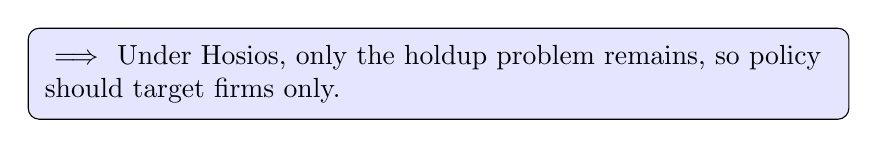
\begin{tikzpicture}
    \node[
        draw,
        rectangle,
        rounded corners,
        fill=blue!10,
        text width=10cm,
        align=left,   % <-- left-align text and let it fill the width
        inner sep=6pt
    ] (box) {
        $\implies$ Under Hosios, only the holdup problem remains, so policy should target firms only.
    };
\end{tikzpicture}
\end{center}
\end{frame}

\begin{frame}{The Empirically Relevant Case: $\eta > \beta$ in Both Sectors}

\textbf{Empirical Evidence:}
\begin{itemize}
\footnotesize 
    \item Matching elasticity: $\eta \approx 0.5$--$0.7$ {\scriptsize (Petrongolo \& Pissarides 2001)}
    
    \item Worker bargaining power: $\beta \approx 0.05$--$0.46$ {\scriptsize (Hagedorn \& Manovskii 2008)}
    
    \item Recent evidence: declining $\beta$ over time {\scriptsize (Azar et al. 2022)}
    
    \item $\Rightarrow$ \textbf{Empirically relevant case: $\eta > \beta$}
\end{itemize}

\vspace{0.3cm}

\textbf{When $\eta > \beta$:} 
\begin{enumerate}
     \item \textit{Capital underinvestment persists} (holdup problem)
    \[k_m^{DE} < k_m^{SP}, \quad k_s^{DE} < k_s^{SP}\]
    
    \item \textit{Excess vacancy creation} in both sectors 
    \[\theta_m^{DE} > \theta_m^{SP}, \quad \theta_s^{DE} > \theta_s^{SP}\]

     % \item \textit{Manufacturing suffers systematic underallocation}
    % \[L_m^{DE} < L_m^{SP}\]
\end{enumerate}
\footnotesize 

% \vspace{0.3cm}

% \textbf{Why?} Manufacturing faces a \textit{double penalty}\\
% \footnotesize 
% Severe capital underinvestment (high capital intensity) $+$ \\ workers under-compensated for matching contribution $\Rightarrow$ distortions compound.

\end{frame}

\begin{frame}{Relevant Case: $\eta > \beta$ in Both Sectors Ctd.}

Deviation from Hosios condition affects $m$ and $s$ sectors \textbf{asymmetrically},  justifying the subsidy on $m$ sector workers' education/skills costs.\\

\vspace{5mm}

\begin{itemize}
%    \item Additional need to 



    \item Balances of marginal increase in training cost and marginal returns from having 1 more worker shifting from $s$ to $m$ : 

    \begin{align*}
        r(\epsilon_m-\epsilon_s) &= \textcolor{red}{\eta} [\theta_mq_mS_m - \theta_sq_sS_s] \quad \text{(SP)}\\
         r(\epsilon_m-\epsilon_s) &= \textcolor{red}{\beta} [\theta_mq_mS_m - \theta_sq_sS_s]  \quad \text{(DE)}\\
    \end{align*}


    \item When $r(\epsilon_m -\epsilon_s)>0$, workers in $m$ need higher payoff than $s$ to compensate for their higher edu. costs. 

    \item If we move from SP to DE, i.e., $\eta \rightarrow \beta$, workers in $m$ suffer a larger welfare loss than those in $s$ and will prefer entering $s$ sector more.  

    \item Hence a subsidy to education cost in $m$ sector is needed to restore DE to SP.
\end{itemize}
\end{frame}




\begin{frame}{Policies to restore DE to SP allocation}
\small

\textbf{a. STEM training subsidy (workers)}: Corrects under-entry into $m$ (education externality).
\medskip

\textbf{b. Investment credit (firms):} Offsets hold-up → raises $K_i/L_i$.

\medskip

\textbf{c. Entry tax (per filled job or vacancy):} Prevents excessive firm entry induced by (b).

\medskip

\medskip 

Overall, expenses and revenues from \textbf{(b)} and \textbf{(c)}  offset each other (fiscal neutral), while \textbf{(a)} requires net fiscal costs.

\medskip

\end{frame}




%===============================================
\section{Calibration and Results}
%===============================================

\begin{frame}{Calibration}
    \begin{table}[h!]
\centering 
\caption{ Parameters.} \label{table_set_parameters}
\begin{adjustbox}{width= 1\columnwidth,center}
 \begin{tabular}{||c c c c||} 
 \hline
 \textbf{Parameter} & \textbf{Description} & \textbf{Value} & \textbf{Source} \\ 
 \hline\hline
   $\rho$ & CES aggregator coefficient & -1 & Boppart (2014) \\ 
%   $m$ & Match Output &  1 & Normalization \\
   $M(u_i,v_i)$ & Matching Function  & u_i^{1/2}v_i^{1/2} & Menzio (2016) \\
   $\beta$ & Worker bargaining power  & 0.5 & Shimer (2005) \\
   $s_s$  & $s$ sector annual separation rate    & 0.20 & BLS \\ 
  $a_m$ & Capital share in manufacturing & 0.74 &  BLS \\
  $a_s$ & Capital share in services & 0.31 &  BLS \\ 
  $A_m$ & Industrial sector technology & 1 &  Normalization \\ 
  $A_s$ & Service sector technology & 1 &  Normalization \\ 
  $\epsilon_m-\epsilon_s$ &  Education cost differential & 0 & ... \\
  $\chi$ & Retirement (annual exit rate) & 0.025 & 40-year working life assumption \\ 
  \hline
  \hline
  $\alpha$ & $m$'s preference weight in final goods & 0.62 & Target industrial employment share \\
  $s_m$ & $m$ sector annual separation rate & 0.06 & Target sectoral unemployment rate \\ 
  $r$ & annual time discount rate  & 0.08 & Target $K/Y$ ratio \\
 \hline
 \end{tabular}
\end{adjustbox}
\end{table}
\end{frame}




\begin{frame}{Decentralized vs. Planner Results }

\begin{table}[H]
 \caption{DE and SP  Allocation under Endogenous Capital Level} \label{DE_SP}
\centering
\begin{adjustbox}{width=0.6\columnwidth,center}

 \begin{tabular}{||c c c||} 
 \hline
 \textbf{Moments} & \textbf{DE} & \textbf{SP} \\  
 \hline\hline
  Real output, $Y$ &  0.487   &  0.588 \\
Capital-to-output ratio, $K/Y$ & 2.508 & 2.860 \\
  Industrial employment, $L_m$ & 19.96\%  & 18.70\% \\
Labor productivity, $A_mf_m(k_m)/A_sf_s(k_s)$ & 5.607 & 6.024\\ 
  Industrial unemploy. rate, $u_m$ & 8.12\% & 9.41\%  \\ 
   Services unemploy. rate,  $u_s$ & 8.14\% & 10.66\%  \\ 
  Relative prices, $p_m/p_s$ & 0.473  &  0.474 \\
%  \textbf{Non-Targeted Moments} &  &  \\
 Relative wages, $w_m/w_s$ &  1.083 & 1.0760 \\
 Relative output, $Y_m/Y_s$ & 1.865  & 1.863 \\
 % Training Expenses/GDP & 0.75\% & 0.75\% \\ 
 [1ex] 
 \hline
 \end{tabular}
\end{adjustbox}
 
\end{table} 

\textbf{Key Takeaways}
\begin{itemize}
  \item  \textbf{Output gains of $~21\%$ from DE → SP,} driven primarily by higher absolute level of capital (hold-up correction); Note $\frac{K}{Y}$ didn't change as much. 
\medskip
         \item \textbf{Lower $L_m$ in SP.} Capital deepening improves labor productivity in $m$ sector more than $s$ sector; the efficient allocation uses more capital and fewer workers in $m$.
\end{itemize}
\end{frame}

\begin{frame}{Quick Quantitative Results}
    \begin{itemize}
\item \textbf{Fiscal costs of turning DE to SP}
\begin{itemize}
\vspace{1mm}
    % \item STEM education subsidy:  about 0.04\% GDP annually
% \vspace{1mm}
    \item Investment subsidy: 0.06\% GDP annually, net cost is zero because it will be financed by taxing firms' employment.

    \vspace{1mm}

    \item Seemly  low fiscal cost because only a fraction of firms/workers need to be subsidized each year at steady state.
\end{itemize}
\color{black}
    \end{itemize}
\end{frame}

\begin{frame}{Extension: Foreign Labor}

\begin{itemize}
    \item \textbf{Motivation:} Some countries actively import skilled foreign workers to support specific sectors (e.g., manufacturing).

    \medskip

    \item \textbf{Experiment (in DE):} Introduce a foreign labor inflow $L_f = 0.1$ that can work only in $m$.

    \medskip

    \item \textbf{Result:} 
    \begin{itemize}
        \item $L_f$ raises total employment in $m$.
        \item Domestic workers reallocate from $m$ to $s$.
        \item In the new steady state:
        \[
        \frac{L_f + L_m'}{L_s'} \;=\; \frac{L_m}{L_s},
        \]
        i.e.\ the overall $m$–$s$ employment ratio is unchanged.
    \end{itemize}

    \medskip

    \item \textbf{Implication:} There is a welfare gain from \emph{saving domestic training costs} for $m$,  
    but importing foreign labor does \emph{not} raise the long‐run manufacturing employment share.
\end{itemize}
    
\end{frame}


%===============================================
\section{Conclusion}
%===============================================
\begin{frame}{Conclusion}
\small
\begin{itemize}

\item Cross-country data show a positive association between STEM enrollment and industry employment.

\medskip


 \item In a search model with capital-intensive manufacturing, the decentralized equilibrium under-invests in capital and yields an inefficiently small manufacturing sector.


\medskip
 \item  In a \textbf{closed economy} setup, the optimal allocation (SP) would have higher capital-output ratio but lower industrial employment share than DE. 


 \medskip

 \item Policies targeting both workers (STEM training) and firms (investment credit, offset by entry tax) can move outcomes toward the planner with manageable fiscal costs.
\end{itemize}
\end{frame}


\begin{frame}
  \centering
  \huge Thank you! \\
  \vspace{1em}
  \normalsize Questions?
\end{frame}

\begin{frame}[allowframebreaks,noframenumbering]{References}
  \bibliography{biblio}
\end{frame}
\end{document}